\documentclass[a4paper,12pt]{article}
\usepackage[T2A]{fontenc}
\usepackage[utf8]{inputenc}
\usepackage[russian]{babel}
\usepackage{graphicx}
\usepackage{float}
\usepackage{amsmath}
\usepackage[margin=2.5cm]{geometry}
\graphicspath{{./}}
\begin{document}
\section*{Приложение. Графики и результаты}

\begin{figure}[H]\centering
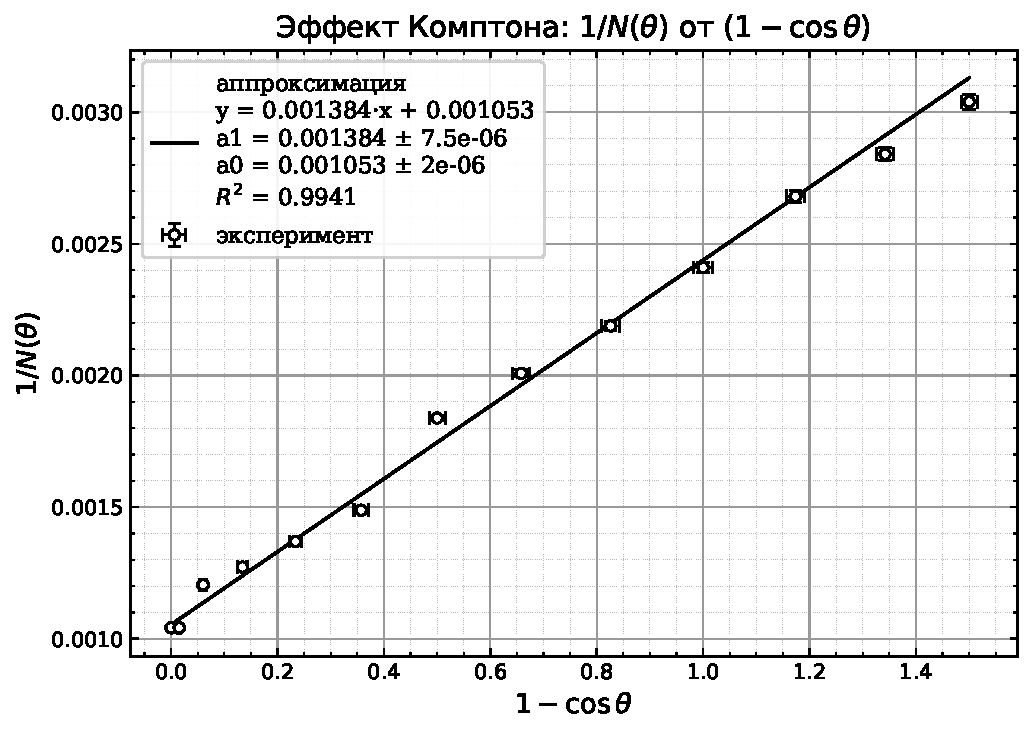
\includegraphics[width=0.82\textwidth]{fig_1_2_compton.pdf}
\caption{Эффект Комптона на графите: $1/N(\theta)$ от $(1-\cos\theta)$; $^{137}$Cs, $E_\gamma=661.657$~кэВ.}
\end{figure}
\begin{center}\small
$A=1.384\times10^{-3}\pm7.5\times10^{-6}$;\quad
$1/N(0)=1.053\times10^{-3}\pm2.0\times10^{-6}$;\quad
$R^2=0.9941$.
\end{center}

\begin{center}\small
\textbf{Наилучшие значения по пересечениям прямой.}
$N_\text{наил}(0)=949.2\pm1.8$;\quad
$N_\text{наил}(90)=410.2\pm1.1$.
\end{center}

\begin{center}\small
\textbf{Энергия покоя электрона.}
$mc^2=E_\gamma\dfrac{N(90)}{N(0)-N(90)}$:\\[2pt]
$\boxed{mc^2=503.5\pm3.3~\text{кэВ}}$;\quad
табличное значение $511.0$~кэВ, отклонение $-1.5\%$ ($2.3\sigma$).
\end{center}

\end{document}
